\documentclass[hyperref={pdfpagelabels=false}]{beamer}
\usepackage{lmodern}
\usepackage{graphicx}%este pacote é para figuras
\usepackage[utf8]{inputenc}
\usepackage[brazil]{babel}% este é para o texto

%\usepackege{multirow,colortbl,array} % estes pacotes são para fazer múltiplas linhas, colorir as celulas e formatar a tabela.

\usepackage{subfig} % este é para fazer sub figuras

\usetheme{Copenhagen}

\title{Mineração de Regras de Associação de Multi-Relação em datasets na Web de Dados}  

\author{Felipe A. Oliveira \\ Orientadores: Maria Cláudia R. Cavalcanti, Ronaldo Ribeiro Goldschmidt e Raquel L. Costa}

\institute {Mestrando em Sistemas e Computação \\ Instituto Militar de Engenharia }

\begin{document}
\begin{frame}
\titlepage
\end{frame} 

\begin{frame}
\frametitle{Tópicos abordados}
\small{\tableofcontents}
\end{frame} 

\section{Introdução}
%densenvolvendo um métodos que realize prerelações de regras sobre um dataset alvo é possível 

\subsection{Motivação}

\begin{frame}
	\frametitle{Motivação}

		\begin{itemize}
        \item Atualmente o mundo tem produzido um volume muito grande de dados \cite{rezende2003mineraccao}. 		
        \item O avanço tecnológico e a utilização das redes sociais permitiu a todos produzir conteúdo. 
        \item  Os sensores presentes nas novas tecnologias produzem dados e informações o tempo todo.
        \begin{figure}[h]
	\centering
		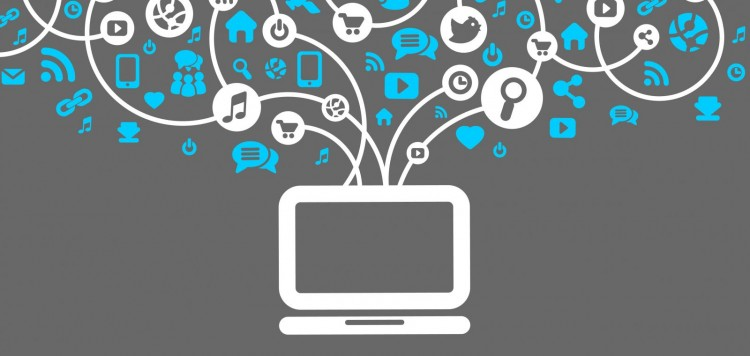
\includegraphics[scale=0.2]{img/produzindodados}
	%\caption{| .}
	\label{fig:produzindodados}
\end{figure}	
     
   
        
% 		\item Segundo \cite{Ramezani2014} minerar regras de associação em banco de dados em grafo, proporciona encontrar regras de associação de multi-relação. 
%         \item Considerando que em um banco de dados em grafo, cada vértice tem um ou mais tipos de relacionamentos, em que cada relação aponta para um outro vértice do grafo. 
%         \item A composição destas relações na direção em que os nós são apontados, trará um entendimento maior sobre o conjunto de informação presento no grafo.
	
	\end{itemize}		
\end{frame}

\begin{frame}
	\frametitle{Motivação}
		\begin{itemize}
        \item O que fazer com essa quantidade gigantesca de dados que estamos produzido? 
	\end{itemize}		
    
    \begin{figure}[h]
	\centering
		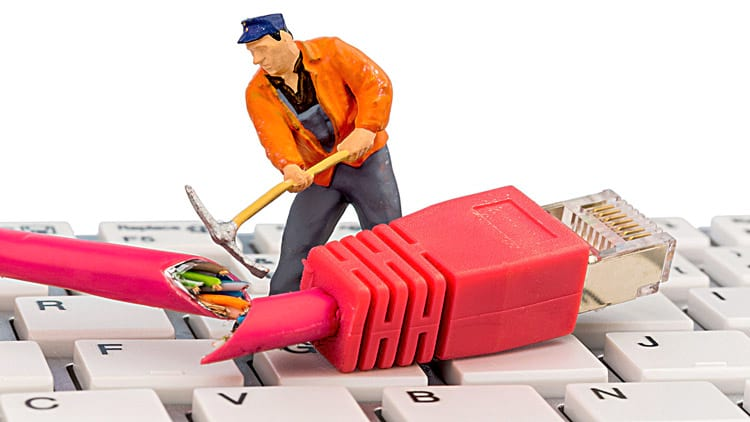
\includegraphics[scale=0.3]{img/internetNao}
	%\caption{| .}
	\label{fig:internetNao}
\end{figure}	
    
    
\end{frame}


\begin{frame}
	\frametitle{Open Data}
		
   Uma medida importante para esses dados, foi torna-los \textbf{disponíveis, abertos e processáveis}, o chamado \textbf{Open Data}.
        \begin{itemize}
        %\item A alguns anos surgiu o movimento "open data", visando tornar público os dados, afim de facilitar a pesquisa.
        \item Dados abertos são aqueles que:
        	\begin{itemize}
        	\item  estão disponíveis para \textbf{qualquer pessoa ou máquina usar}, não importando o fim;
            \item não tem \textbf{nenhum custo} para sua utilização; 
            \item tem como contrapartida apenas \textbf{dar o crédito a fontes}.
%(http://bigdatarevolution.blogspot.com.br/2014/02/open-data-day-um-convite-para-ouvir-e.html) 
			\end{itemize}
        \item No Brasil, a \textbf{lei de acesso a informação} (Nº 12.527, DE 18 DE NOVEMBRO DE 2011), \textbf{tornou acessível os  dados governamentais}, que a partir de então deveriam estar \textbf{disponíveis sem restrições} \cite{Vaz2011}, como é possível ver no PORTAL BRASILEIRO DE DADOS ABERTOS (http://dados.gov.br/).
	\end{itemize}		
\end{frame}

\begin{frame}
	\frametitle{Linked Open Data (LOD)}
Com os dados disponíveis é preciso buscar formas de entende-los.
\begin{itemize}

	\item A LOD além de tornar os dados abertos e provessáveis, \textbf{busca ligar esses dados}, possibilitando dizer que \textbf{se um dado é encontrado num dataset}, certamente \textbf{um outro dataset terá o mesmo dado ou alguma informação complementar sobre ele}. \cite{bizer2009linked}
        \item O Padão RDF é utilizado na LOD, pois \textbf{com suas triplas (sujeito, predicado e objeto) é possível construir uma estrutura de grafo} e apontar a direção onde a informação será melhor descrita.
    
	\end{itemize}		
\end{frame}


\begin{frame}
\frametitle{Web de Dados}
Com os dados na Web de Dados é possível:
\begin{itemize}
  
   \item Realizar analises;
   \item Fazer mineração de dados; 
   \item Obter conhecimento. 
\end{itemize}
\end{frame}

\begin{frame}
	\frametitle{Mineração de regras de associação}
		\begin{itemize}
        \item  Existem várias \textbf{maneiras de realizar análises} (tarefas de mineração), como vista em \cite{Camilo2009}, \textbf{entre elas a mineração de regras de associação}.
     \item Com esse tipo de análise \textbf{é possível descobrir que}:
     \begin{itemize}
     \item Um dado ator de filmes pode atuar em filmes de um dado diretor ou ter uma frequência grande de coautoria;
     \item Com o Dataset D1 e outro dataset interligado, D2,  posso navegar pela interligacao entre os dois e encontrar novas associações.
	\end{itemize}
    \end{itemize}		
\end{frame}


\subsection{Problema}
 
\begin{frame}
	\frametitle{Problema}	
		\begin{itemize}
	%	\item Utilização do banco de dados de gerenciamento de coleções botânicas do Jadim Botânico do Rio de Janeiro (JBRJ) JABOT.
	%	\item Modelagem em grafo do JABOT.
	\item \cite{tavares2015} mostra que o \textbf{crescimento do número de fontes na Web de Dados} tem motivado o desenvolvimento de aplicações e ferramentas que consomem o conteúdo disponibilizado por estas fontes. 
    \item Porém, \textbf{estas aplicações}, em geral, \textbf{utilizam datasets específicos}, o que \textbf{limita a quantidade de informação}, pois só são obtidas através dos resultados das consultas.      
    
    %\item {Muitos datasets estão sendo publicados na web de dados com a tendencia de aumentar.\cite{tavares2015} }
	\end{itemize}		
\end{frame}
 
\begin{frame}
	\frametitle{Problema}
	\begin{figure}[h]
	\centering
		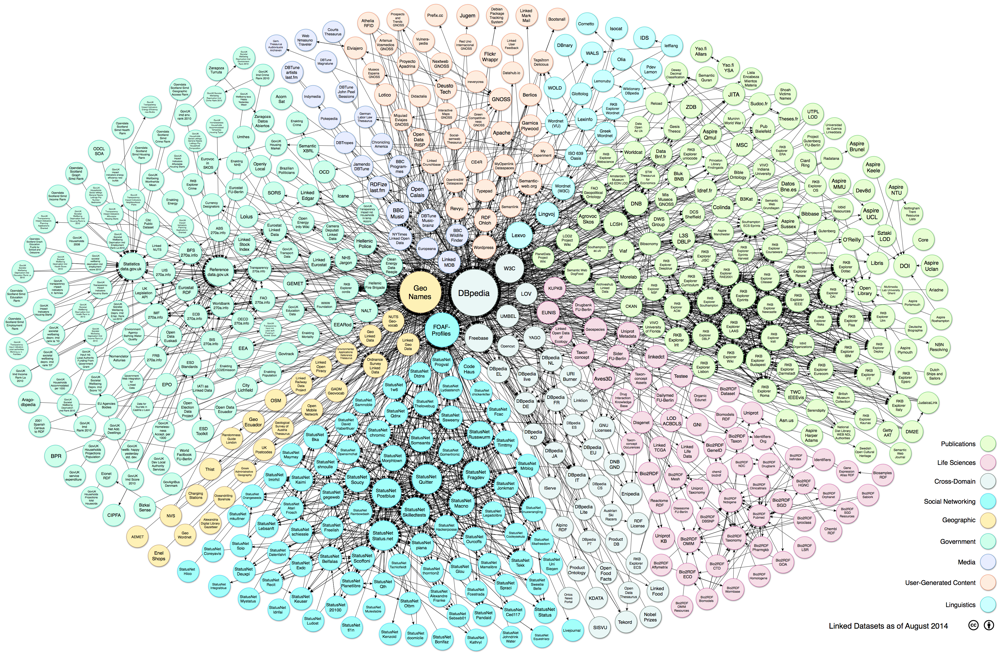
\includegraphics[scale=0.2]{img/lod-cloud_colored_1000px}
	\caption{| Diagrama da nuvem do Linking Open Data em 2014 (Fonte: http://lod- cloud.net/).}
	\label{fig:lod-cloud_colored_1000px}
\end{figure}	
\end{frame}

\begin{frame}
	\frametitle{Problema}
Com o \textbf{crescimento do número de datasets}, torna-se necessário:
\begin{itemize}
	\item  \textbf{Realizar analises} sobre esses dados que estão espalhados na Web de Dados.
 	\item Descobrir se é possível \textbf{densenvolver métodos que realizem prerelações de regras} sobre um dataset alvo.
	\end{itemize}		
\end{frame}

%Retiramos essa parte pois, parece que esse tipo de comentário pode desconstruir o discurso todo, já que estamos considerando a existencia de ligações entre os data set, falar que existe carencia de ligação nao convem.
% \begin{frame}
% 	\frametitle{Problema}
% 	\begin{itemize}
% 	\item Dentro de um mundo de datasets um dos problemas é a \textbf{Carência de ligações entre eles} \cite{Travassos2014}. 
%     \item Já que esses datasets tem sua área de domínio específico, a existencia de ligações entre eles possibilitaria novas analises.
% 	\end{itemize}		
% \end{frame}


\begin{frame}
	\frametitle{Problema}
	\begin{itemize}
	\item { \textbf{Os algoritmos existentes são de alta complexidade}, como os apresentados por \cite{Ramezani2014} e \cite{Elseidy2014}.}
    \item Eles \textbf{demandam um elevado poder de processamento}, tornando inviável sua aplicação na Web de Dados. 
	\end{itemize}		
\end{frame}

\begin{frame}
	\frametitle{Problema}
	\begin{itemize}
	\item {Como \textbf{viabilizar a analise} sobre a Web de Dados de modo a \textbf{encontrar novas ligações} e \textbf{extrair conhecimento útil}?}
	\end{itemize}		
\end{frame}


\subsection{Hipótese}
 
\begin{frame}
	\frametitle{Hipótese}
	
		\begin{itemize}
	 \item Será que podemos \textbf{criar um método} que a partir das pre-relacões de um dataset alvo, seja possível \textbf{reduzir e tornar viável a análise} sobre outros datasets interligados, \textbf{direcionando essa análise} para as conexões com \textbf{maior potencial de descobertas}?
	
%       \item Será que densenvolvendo um métodos que realize prerelações de regras sobre um dataset alvo é possível encontrar pontos de enriquecimento?
%   	\item Será que haveria uma forma de reduzir o conjunto de dados ligados a considerar, buscando direcionar a análise para as conexoes com maior potencial para descobertas?

	\end{itemize}		
\end{frame}


\subsection{Objetivo}
 
\begin{frame}
	\frametitle{Objetivo}
		\begin{itemize}
	    \item Desenvolver um método para viabilizar a analise sobre a Web de Dados de modo a reduzir a quantidade de dados a ser analisado e encontrar novas ligações que enriquecerão o dataset alvo. 
	\end{itemize}		
\end{frame}

\section{Conceitos Básicos}

\begin{frame}
\frametitle{Conceitos Básicos}
Para atingir esse objetivo, veremos alguns conceitos básicos:
\begin{itemize}
  \item Web de Dados;
  \item Datasets;
  \item RDF;
  \item Links Externos;
  \item Mineração de regras de associação;
  \item Mineração de regras de associação de multi-relação.
 
\end{itemize}
\end{frame}



\begin{frame}
\frametitle{Web de Dados e Datasets}
\begin{itemize}
  \item{A Web Semântica ou Web de Dados \textbf{é composta por dados, títulos, identificações, propriedades e quaisquer outros dados que se possa produzir}.}
  \item Os datasets nessa Web de dados \textbf{são conjuntos de dados RDF que são disponibilizados sobre um domínio  de conhecimento.}
  \begin{itemize}
  \item Exemplo de dataset: DBpedia, construída a partir da Wikipedia, que \textbf{fornece dados sobre pessoas, lugares, filmes e outros}. 
  \end{itemize}
  %\item{As tecnologias da Web Semântica (RDF, OWL, SPARQL) fornecem um ambiente onde uma aplicação pode consultar/analisar esses dados e fazer inferências usando vocabulários controlados \cite{Paletta2015}.}
\end{itemize}
\end{frame}

% \begin{frame}
% \frametitle{Web de dados}
% \begin{figure}[h]
% 	\centering
% 		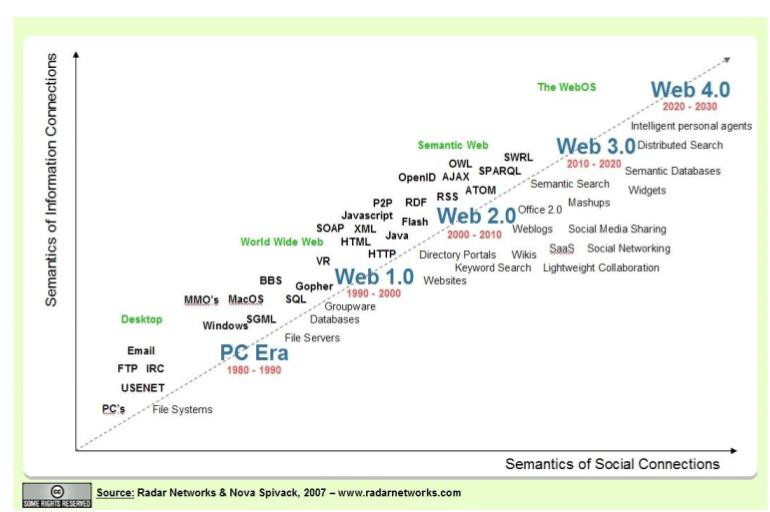
\includegraphics[scale=0.3]{img/O_Futuro_da_Web_Sem_ntica}
% 	\caption{| O Futuro da Web Semântica \cite{Paletta2015}}
% 	\label{fig:O_Futuro_da_Web_Sem_ntica}
% \end{figure}
% \end{frame}

% \begin{frame}
% \frametitle{Web de dados}
% \begin{figure}[h]
% 	\centering
% 		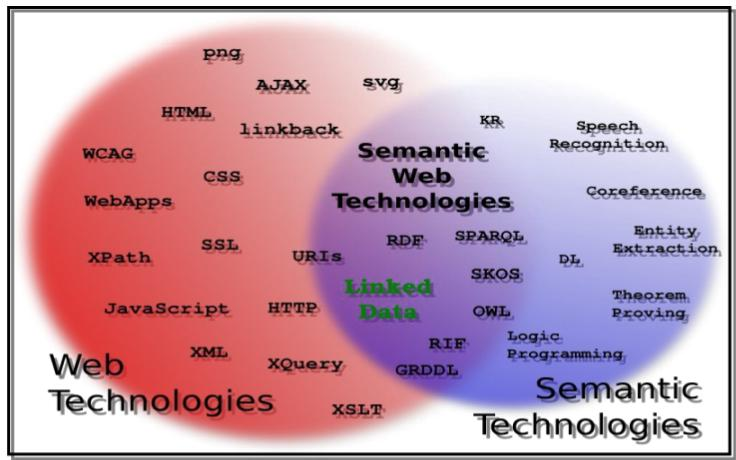
\includegraphics[scale=0.3]{img/Linked_Data_-_Contexto_Tecnol_gico}
% 	\caption{| Linked Data - Contexto Tecnológico \cite{Paletta2015}}
% 	\label{fig:Linked_Data_-_Contexto_Tecnol_gico}
% \end{figure}
% \end{frame}



% \begin{frame}
% \frametitle{Datasets}

% \begin{itemize}
% 	\item {Datasets são conjuntos de dados RDF que são disponibilizados sobre um domínio  de conhecimento.}
%     \item {Os datasets permitem o acesso ao seu conteúdo por meio de Web crawling, RDF dump ou via um SPARQL endpoint.  \cite{tavares2015}}
% \end{itemize}	
% Exemplo de dataset: DBpedia, construída a partir da Wikipedia, que fornece dados sobre pessoas, lugares, filmes e outros.    
% \end{frame}




\begin{frame}
\frametitle{RDF (Resource Description Framework)}
\begin{itemize}
  \item{O modelo RDF é \textbf{representado por meio de triplas}. 
  \item Essas triplas podem ser organizadas como um grafo direcionado.}
  \item Os componentes das triplas são: \textbf{Sujeito, Predicado e Objeto}. 
  \begin{itemize}
  		\item sujeito é o recurso descrito; 
        \item o objeto pode ser um valor literal ou um recurso relacionado ao sujeito; 
        \item o predicado indica a relação que existe entre o sujeito e o objeto.
  \end{itemize}    
 \item Cada item é \textbf{identificado por uma URI} interna ou externa. \cite{tavares2015}
\end{itemize}  
\end{frame}

\begin{frame}
\frametitle{Exemplo de tripla RDF}
\begin{itemize}
 \item{ Essa Figura mostra uma tripla RDF, indicando em qual cidade se localiza a Universidade Federal de Pernambuco. }
\end{itemize}  

\begin{figure}[h]
	\centering
		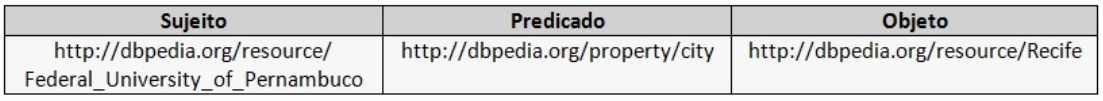
\includegraphics[scale=0.3]{img/tripla_RDF_DBpedia}
	\caption{|Tripla RDF DBpedia}
	\label{fig:tripla_RDF_DBpedia}
\end{figure}
\end{frame}



\begin{frame}
\frametitle{Links Externos}
\begin{itemize}
  \item{A Web de Dados \textbf{pode ser acessada usando navegadores Linked Data}, da mesma forma que a Web tradicional é acessada usando navegadores HTML.}
  \item{No entanto, em vez de seguir ligações entre páginas HTML, navegadores Linked Data \textbf{permitem que os usuários naveguem entre diferentes fontes de dados seguindo os links RDF}.}
  \item{Assim o usuário inicia o processo de busca com uma fonte de dados e, em seguida, \textbf{move-se através de uma potencial e interminável fontes de dados WEB}, conectados por esses links RDF. \cite{Paletta2015} }
\end{itemize}  
\end{frame}


\begin{frame}
\frametitle{Links Externos}
\begin{figure}[h]
	\centering
		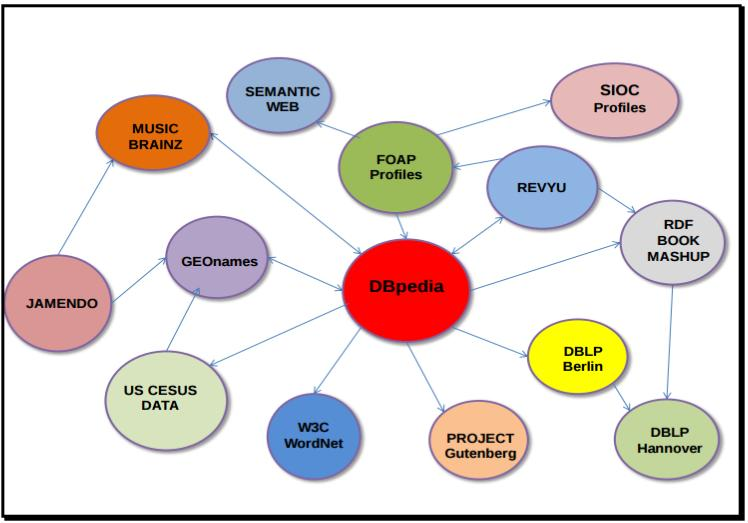
\includegraphics[scale=0.3]{img/Linking_Open_Data_em_um_Projeto_DBpedia}
	\caption{| Linking Open Data em um Projeto DBpedia \cite{Paletta2015}}
	\label{fig:Linking_Open_Data_em_um_Projeto_DBpedia}
\end{figure}
\end{frame}

\begin{frame}
\frametitle{KDD - Knowledge Discovery in Databases}
\begin{itemize}
  \item{\cite{Fayyad1996} destacam os passos aplicados para o processo de transformação de dados em conhecimento.}
\end{itemize}
\begin{figure}[h]
	\centering
		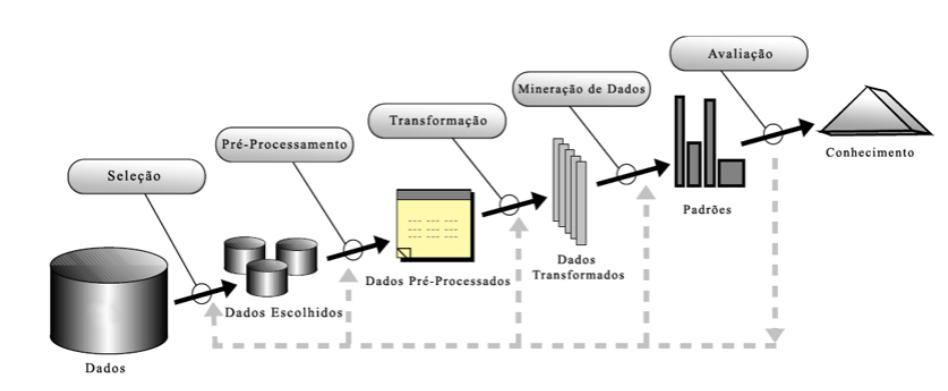
\includegraphics[scale=0.3]{img/Processo_de_KDD.jpg}
	\caption{| Representação do processo de KDD \cite{Fayyad1996}}
	\label{fig:Processo_de_KDD}
\end{figure}
\end{frame}


\begin{frame}
\frametitle{Mineração de regras de associação}
\begin{itemize}	
      \item { O conceito de itens frequentes é apresentado por \cite{Agrawal1993}, onde esse conjuntos de "Frequent Itemset" é criado respeitando um valor mínimo para cada item. }
      \item { Com esses conjuntos é possível minerar regras de associação. }
	  \item { Para cada regra gerada é aplicado um suporte (MinSup) e confiança (MinCon) mínima, obtendo assim resultados válidos.  }
\end{itemize}	
\end{frame}


\begin{frame}
\frametitle{Mineração de regras de associação de multi-relação}
\begin{itemize}
  \item{ \cite{Ramezani2014} apresenta um \textbf{novo conceito: Regras de associação de multi-relação}, denominado 'MRAR' que \textbf{diferente das regras de associação clássicas} (geralmente extraídas  de banco de dados relacionais), \textbf{diz que cada item da regra consiste em uma entidade e várias relações}.  }
  %\item Para garantir que as regras encontradas são válidas, aplica-se o Minsup e MinConf, como vista no modelo clássico.
  %\item A novidade para utilização do MRAR são os \textbf{"EndPoints" (vértices que recebem alguma aresta)}. 
%   \item{As relações indicam um relacionamento indireto entre as entidades.}
\end{itemize}
\end{frame}


\begin{frame}
\frametitle{Mineração de regras de associação de multi-relação}
Ex: Regra de associação de Multi-Relação, onde o primeiro item consiste em três relações Live-In, near-by e climate-type

% ("Aqueles que vivem em um lugar que é perto de uma cidade com tipo de clima húmido e também tem menos que 20 anos -$>$ sua condição de saúde é bom")

	\begin{figure}[h]
	\centering
		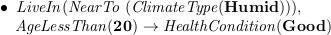
\includegraphics[scale=0.8]{img/exemplo}
	\caption{ Exemplo de Regra de Associação de Multi-Relação}
	\label{fig:exemplo}
\end{figure}	

\end{frame}



\section {Trabalhos relacionados}

\begin{frame}
	\frametitle{Trabalhos relacionados}
\begin{itemize}
      \item {Em \cite{Hendrickx2015} é proposto uma forma minerar regras de associação entre rótulos de nó no grafo, descobrindo assim informações adicionais sobre as correlações e interações entre eles. %Apresentam um algoritmo que descobre regras que permitem afirmar que, se um conjunto de rótulos é encontrado em um gráfico, há uma alta probabilidade de que algum outro conjunto de rótulos possam ser encontrados nas proximidades. Descobrindo a regra que diz que, se um nó com rótulo X está ligado a algum lugar no grafo de entrada, há uma alta probabilidade de que os rótulos em Y sejam encontrados nas proximidades.
      }

	\end{itemize}
    Trabalha com os rótulos dos nós, mas não leva em consideração os vários tipos de relacionamento presentes no grafo.
\end{frame}

\begin{frame}
	\frametitle{Trabalhos relacionados}
\begin{itemize}
	\item Em \cite{Elseidy2014} é apresentado o GRAMI (GRAph MIning), para a \textbf{mineração de subgrafos frequentes num único grafo grande}. Mostra uma abordagem que \textbf{encontra os conjuntos mínimos de frequência e evita a enumeração custosa de todos os casos}.
 	%\item GRAMI faz a avaliação de modelos frequentes como um problema de satisfação de restrições (CSP - constraint satisfaction problem). Em cada iteração, GRAMI resolve o CSP até encontrar o conjunto mínimo de nós que são suficientes para avaliar a frequência do subgrafo, e ignora todas as aparências restantes.
	\end{itemize}	
	Entretanto não atendem aos dados da Web de Dados.
\end{frame}


% \begin{frame}
% 	\frametitle{Trabalhos relacionados}
% \begin{itemize}
%       \item{\cite{Nebot2012} investiga casos de ontologias expressas em OWL combinadas em transações, com o objetivo de ser processadas por algoritmos tradicionais \cite{Agrawal1993}, e como seria o rico conhecimento codificado nas respectivas ontologias para reduzir o espaço da busca. }
% 	\end{itemize}		
% \end{frame}


\begin{frame}
	\frametitle{Trabalhos relacionados}
\begin{itemize}
	\item \cite{Ramezani2014} \textbf{propõe um algoritmo para minerar regras de associação em banco de dados em grafo}, visando encontrar regras de associação de multi-relação. 
    \item Considerando que em um banco de dados em grafo, \textbf{cada vértice tem um ou mais tipos de relacionamentos}, em que cada relação aponta para um outro vértice do grafo, \textbf{a composição destas relações na direção em que os nós são apontados, traz um entendimento maior sobre o conjunto de informação presente no grafo}.
	\end{itemize}		
\end{frame}

\begin{frame}
\frametitle{Trabalhos relacionados}
\begin{figure}[h]
	\centering
		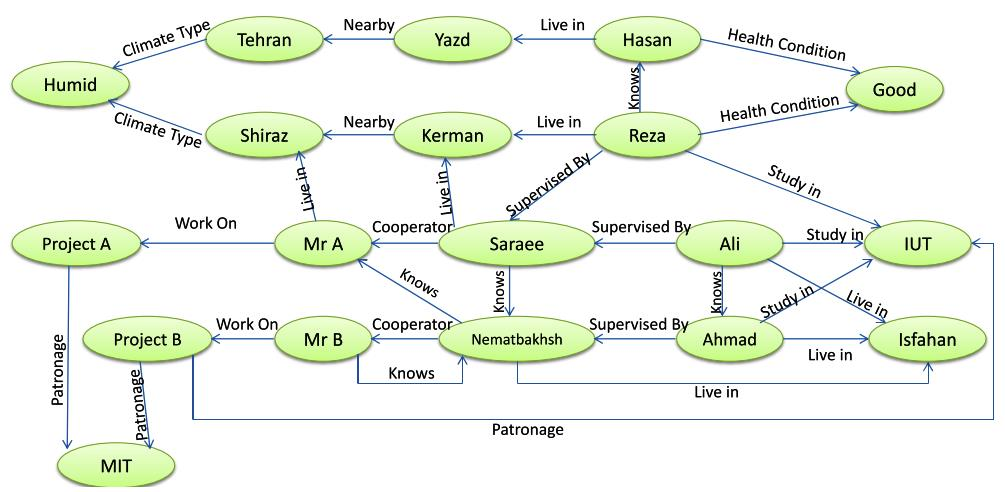
\includegraphics[scale=0.3]{img/Graph}
	\caption{| Um exemplo de um grafo direcionado com rótulo nas arestas \cite{Ramezani2014}}
	\label{fig:Graph}
\end{figure}
\end{frame}



% \begin{frame}
% \frametitle{Trabalhos relacionados}
% \begin{figure}[h]
% 	\centering
% 		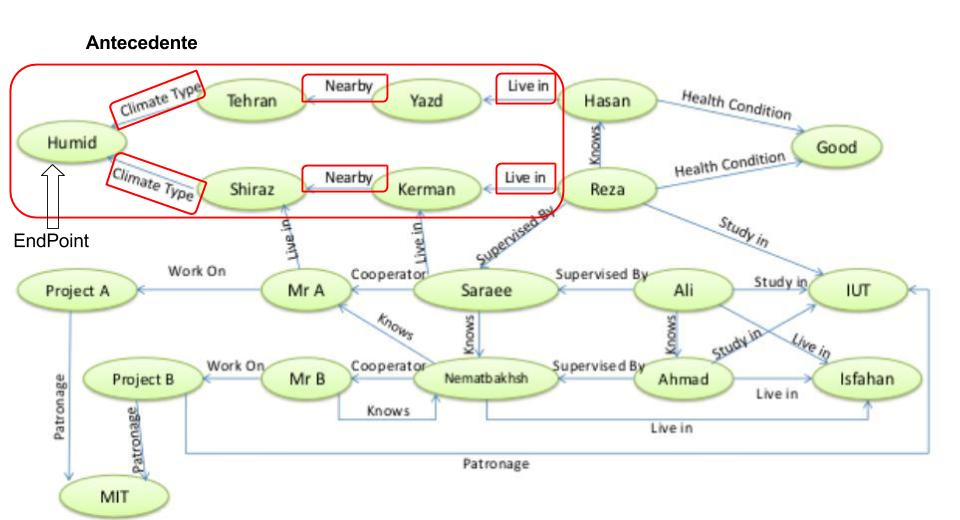
\includegraphics[scale=0.3]{img/Grafico_MRAR_1}
% 	\caption{| Antecente de uma Regra de associação de Multi-Relação.}
% 	\label{fig:Grafico_MRAR_1}
% \end{figure}
% \end{frame}

\begin{frame}
\frametitle{Trabalhos relacionados}
\begin{figure}[h]
	\centering
		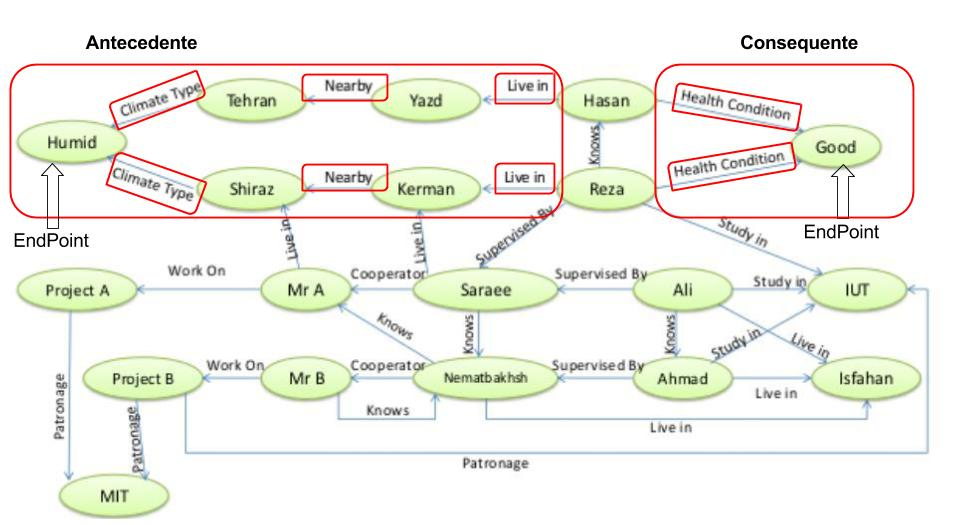
\includegraphics[scale=0.3]{img/Grafico_MRAR_2}
	\caption{| Antecente e consequente de uma Regra de associação de Multi-Relação.}
	\label{fig:Grafico_MRAR_2}
\end{figure}
\end{frame}



\begin{frame}
	\frametitle{Trabalhos relacionados}
\begin{itemize}
%       \item Considerando a regra que indica que aqueles que têm o estado de saúde bom vivem perto de uma cidade que tem o clima úmido.
      
% | Health Condition(Good) -$>$Live In(Near by(Climate Type(Humid))) -- Hasan and Reza


\item Na figura anterior temos que:
	\begin{itemize}
    \item {Humid e Good são entidades endpoint.}
    \item {Live-In, Near-by, Climate-Type e Health-Condition são relações intermediárias. }  
    \item Yazd, Tehran, Shiraz e Kerman são entidades intermediárias
    \item Hasan e Reza são as entidades que  satisfazem a regra.
	\end{itemize}
\end{itemize}
\end{frame}


\begin{frame}
\frametitle{Trabalhos relacionados}
\begin{itemize}
\item O trabalho de \cite{Ramezani2014} foi o mais próximo, porem ele não faz o que queremos fazer (quando pensamos na interligação de datasets).
\end{itemize}		
\end{frame}


    
\section{Proposta}

\begin{frame}
\frametitle{Recordando o objetivo do trabalho}
\begin{itemize}
 \item Desenvolver um método para viabilizar a analise sobre a Web de Dados de modo a reduzir a quantidade de dados a ser analisado e encontrar novas ligações que enriquecerão nosso dataset alvo. 
\end{itemize}		
\end{frame}


    

  \subsection{Visão Geral}  
	\begin{frame}
    \frametitle{Visão Geral}
   \begin{itemize}
      	\item Tendo como base um dataset de domínio/conhecimento específico em RDF, espera-se que ao realizar a mineração de regra de associação de multi-relação, \textbf{os consequentes das regras encontradas, servirão como ponte para outros datasets de domínios diferentes através de seus links externos}.
        \item Dessa maneira \textbf{poderemos enriquecer nosso dataset com informações úteis}, ampliando assim seu conhecimento, possibilitando \textbf{encontrar novas regras e evitando ter que minerar o segundo dataset por completo}. 
    \end{itemize}
   
   
	\end{frame}
    
	\begin{frame}
    \frametitle{Visão Geral}
    \begin{figure}[h]
	\centering
		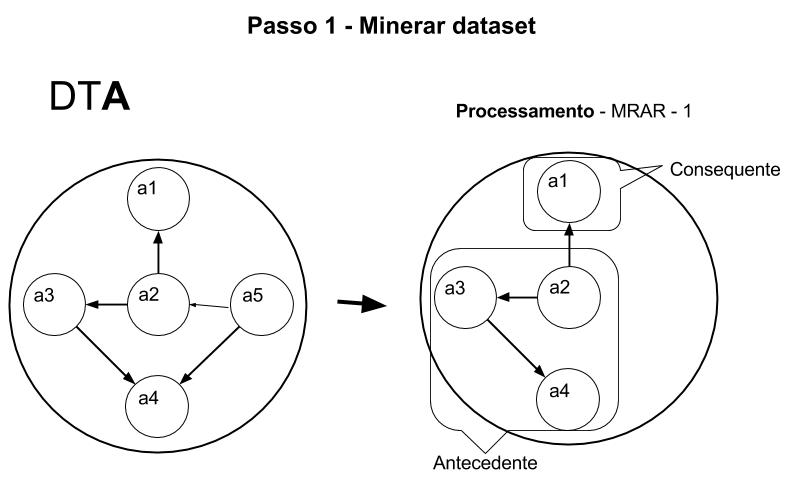
\includegraphics[scale=0.3]{img/VisaoGeralProposta1}
	\caption{| Processo para estender o conhecimento de um datasets - Passo 1.}
	\label{fig:VisaoGeralProposta1}
\end{figure}
	\end{frame}
    
       
	\begin{frame}
    \frametitle{Visão Geral}
    \begin{figure}[h]
	\centering
		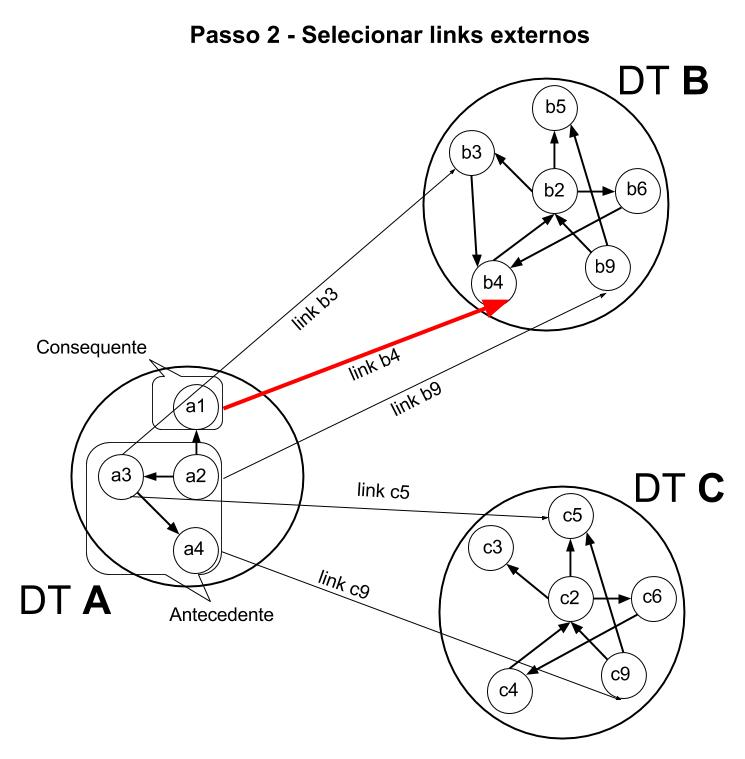
\includegraphics[scale=0.2]{img/VisaoGeralProposta2}
	\caption{| Processo para estender o conhecimento de um datasets - Passo 2.}
	\label{fig:VisaoGeralProposta2}
\end{figure}
	\end{frame}
       
	\begin{frame}
    \frametitle{Visão Geral}
    \begin{figure}[h]
	\centering
		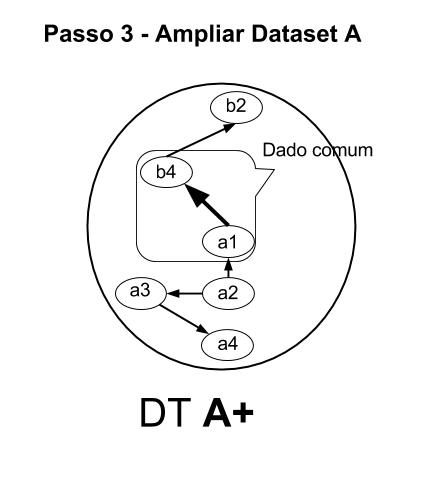
\includegraphics[scale=0.3]{img/VisaoGeralProposta3}
	\caption{| Processo para estender o conhecimento de um datasets - Passo 3.}
	\label{fig:VisaoGeralProposta3}
\end{figure}
	\end{frame}
       
	\begin{frame}
    \frametitle{Visão Geral}
    \begin{figure}[h]
	\centering
		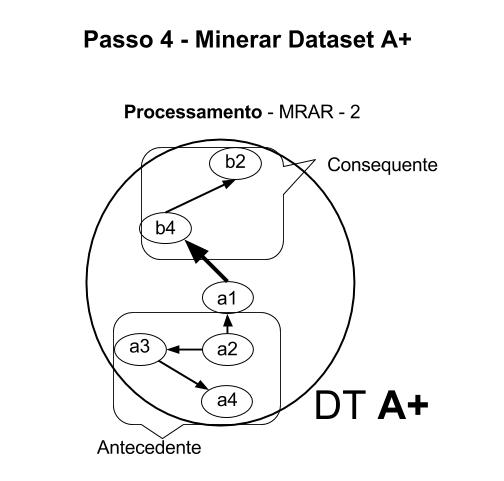
\includegraphics[scale=0.3]{img/VisaoGeralProposta4}
	\caption{| Processo para estender o conhecimento de um datasets  - Passo 4.}
	\label{fig:VisaoGeralProposta4}
\end{figure}
	\end{frame}
    
    
    
\subsection{Estudo de caso - Jabot}  


\begin{frame}
   \frametitle{Estudo de caso}
	Para o estudo de caso vamos  \textbf{utilizar as informações do banco de dados de gerenciamento de coleções botânicas do Jardim Botânico do Rio de Janeiro (JBRJ)}, chamado de  \textbf{JABOT} (http://jabot.jbrj.gov.br/).
    
   No Jabot temos:
    \begin{itemize}
        	\item Informações sobre a biodiversidade;
            \item Dados da ocorrência de plantas, fungos e algas, além de informações sobre DNA, madeira e fruto.
	\end{itemize}
\end{frame}


\begin{frame}
   \frametitle{Estudo de caso}
	
    Itens que estão em desenvolvimento:
    \begin{itemize}
    	\item Modelagem e construção dos Jabot em grafo (JabotG);
            \item Implementação do Algoritmo MRAR de \cite{Ramezani2014}.
	\end{itemize}
\end{frame}
    
    
    
	\begin{frame}
    \frametitle{Estudo de caso}
    \begin{figure}[h]
	\centering
		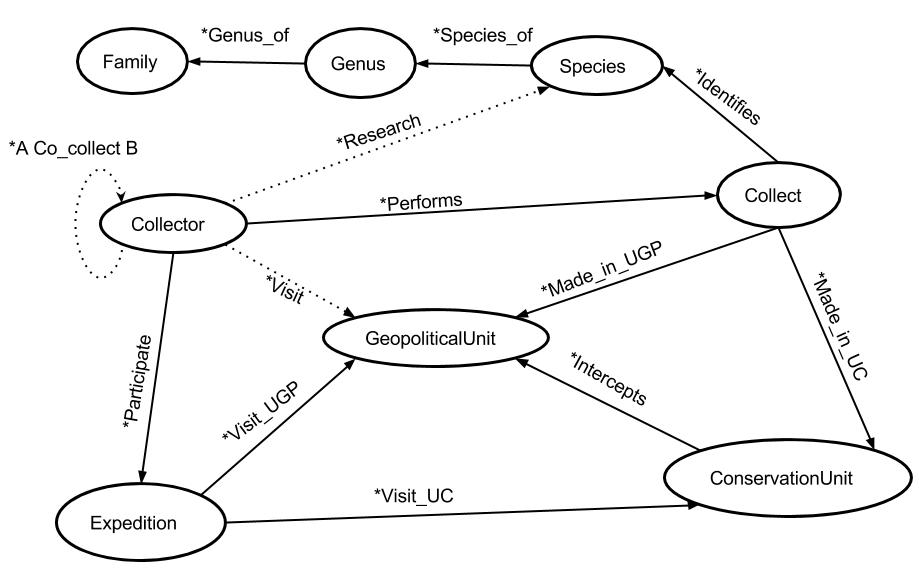
\includegraphics[scale=0.3]{img/SchemeJabot_-_Grafo}
	\caption{| Modelagem JabotG.}
	\label{fig:SchemeJabot_-_Grafo}
\end{figure}
	\end{frame}    
    
    
  \subsection{Metodologia}  
	\begin{frame}
    \frametitle{Metodologia}
     \begin{itemize}
        	\item Revisão da Literatura
            \item Concepção da abordagem proposta
            \item Escolha de técnicas e métodos para implementação
            \item Implementação do Algoritmo MRAR
            \item Experimentos preliminares com o dataset de  \cite{Ramezani2014}
            \item Implementação da abordagem proposta
           	\item Modelagem e conversão do BD Jabot relacional em Grafo 
			\item Aplicar a abordagem proposta aos dados do JabotG
			\item Realização de experimentos e validação dos resultados
		\end{itemize}
	\end{frame}
    
    
\begin{frame}
\frametitle{Cronograma}
\begin{figure}[C] 
	\centering
		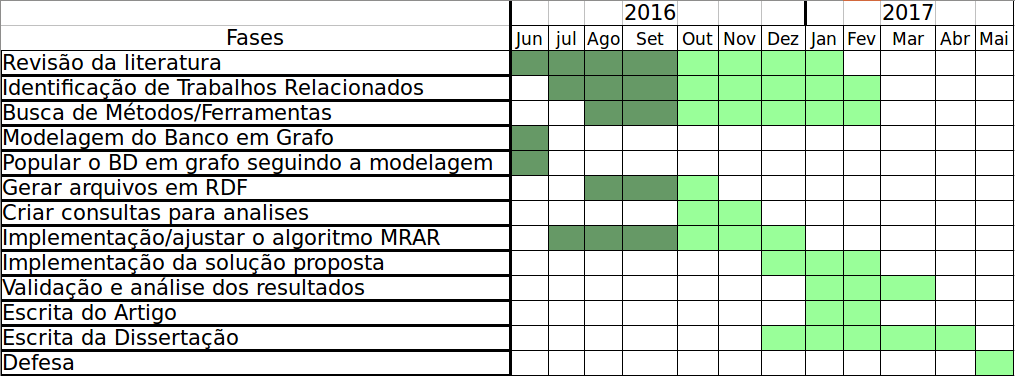
\includegraphics[scale=0.3]{img/Cronograma.png}
	\caption{Cronograma até a Defesa.}
    
	\label{fig:Cronograma}
\end{figure}
\end{frame}



\section {Referências}
\begin{frame}
\frametitle{Bibliografia}
    \bibliographystyle{apalike}
    \small{ \bibliography{ref} }
\end{frame}

\end{document}

